\documentclass[11pt,a4paper]{article}

% ---------------------------------------------------------------------------
% Objective 3 report: routing, harness-run tools, guided discovery and a faster answer path
% Compile with:  pdflatex objective3_report.tex  (run twice for references)
% Figures are expected in ./figs/ (produced by make_figs.py).
% ---------------------------------------------------------------------------

\usepackage[margin=2.4cm]{geometry}
\usepackage[T1]{fontenc}
\usepackage{mathpazo}
\usepackage{microtype}
\usepackage{graphicx}
\usepackage{booktabs}
\usepackage{tabularx}
\usepackage{xltabular}
\usepackage{array}
\usepackage{multirow}
\usepackage{xcolor}
\usepackage{enumitem}
\usepackage{amsmath,amssymb}
\usepackage{caption}
\usepackage{float}
\usepackage{tikz}
\usetikzlibrary{arrows.meta,positioning,shapes.geometric,fit,calc}
\usepackage[hidelinks]{hyperref}

\definecolor{ink}{HTML}{0B0B0B}
\definecolor{ink2}{HTML}{52514E}
\definecolor{qblue}{HTML}{2A78D6}
\definecolor{qorange}{HTML}{EB6834}
\definecolor{qaqua}{HTML}{1BAF7A}
\definecolor{qred}{HTML}{C9302C}
\definecolor{boxfill}{HTML}{F3F7FD}
\definecolor{fixfill}{HTML}{EEF7EE}

\captionsetup{font=small,labelfont=bf}
\setlist{itemsep=2pt,topsep=4pt}
\renewcommand{\arraystretch}{1.18}
\newcolumntype{L}{>{\raggedright\arraybackslash}X}
\newcommand{\met}{\textcolor{qaqua}{\textbf{met}}}
\newcommand{\missed}{\textcolor{qred}{\textbf{missed}}}
\newcommand{\na}{\textcolor{ink2}{n/a}}

% Placeholder: replace before submission
\newcommand{\placeholder}[1]{\textcolor{red}{[#1]}}
\newcommand{\reportdate}{15 October 2026}

\title{\textbf{Routing, Kiosk-Run Tools and Guided Discovery\\for a Small-Model Retail Kiosk Assistant}\\[4pt]
\large Objective 3: Tools, Guided Discovery and a Faster Answer Path}
\author{Anany Dev Choudhary\\\small Roll No.\ 228070135\\\small Department of Electrical Engineering\\\small Indian
Institute of Technology Kanpur}
\date{\reportdate}

\begin{document}
\maketitle

\begin{abstract}
\noindent
Objective~2 grounded an offline watch-store kiosk assistant in store knowledge, but left it slow, prone to looping
through tool calls, worse on tool tasks than without retrieval, and still hallucinating on questions it could not
answer. Objective~3 keeps both models fixed (Qwen3.5-2B on a CPU-only kiosk, Qwen3.5-4B on an integrated GPU) and changes
everything around them. An intent router sends each message down the cheapest path that can answer it; the kiosk itself
runs lookups, stock checks, comparisons and staff hand-offs; a slot-filling policy guides shoppers to a recommendation;
fixed replies, an entity check and an answer check guard the knowledge path; follow-ups keep the watch in focus; and
the retrieval and generation steps were made faster. Thirteen changes were tried on development data, each kept or dropped
by a rule written before its run, and the result (O3-final) was confirmed once on a fresh test set of 775 cases and
60 simulated shopping dialogues.
On the test set, O3-final answers \textbf{69.6\% of store questions against 51.9\%} for Objective~2's setup on the 2B
(+17.7 points) and \textbf{77.6\% against 62.5\%} of tool cases (+15.1), cuts the 2B's wait for a tool reply by about
22\,s on the laptop CPU, and turns the shopping dialogues from 63--87\% to 97\% fit with what the customer asked for,
on both models. The pre-registered confirmation holds for the 4B (follow-ups 66.7\% to 90.0\%, nothing worse) and
fails for the 2B on one rule: its follow-up gain (+10 points) is a tie after correcting for six tests. An ablation of
the whole path on the test set attributes the gains step by step and shows the router alone is worth +14 to +28 points
on tool cases, follow-ups and dialogues for the 2B. Fourteen of 24 success criteria are met for the 2B and 13 of 23 for
the 4B. The hallucination target is missed by a wide margin: a blind judge finds unsupported claims in 23\% (4B) and
37\% (2B) of replies to unanswerable questions, no better than Objective~2's setup, and the 2B's Hinglish replies are the
weakest. These, and the failures found on the test set, are the training targets of Objective~4.
\end{abstract}

\tableofcontents
\vspace{6pt}
\hrule

% ===========================================================================
\section{Introduction}\label{sec:intro}
% ===========================================================================

\subsection{Where Objective 2 left the assistant}
The assistant answers customers at an in-store kiosk of a fictional watch retailer, Veyra, entirely offline. Objective~1
selected the two models and the seven catalogue tools; Objective~2 added a retrieval pipeline over an 812-chunk store
knowledge corpus and a fallback that refuses when nothing relevant is found. Objective~2's deployed setup, which this
report calls \textbf{O3-B0}, left five problems:
\begin{itemize}
  \item \textbf{Hallucination} on questions the store information cannot answer: 19\% (4B) and 23\% (2B) of replies,
        against a 5\% target, and up to 48\% on harder subsets.
  \item \textbf{A regression on tool tasks}: with retrieval on every message, tool cases fell from 78\% to 72\% (4B) and
        from 69\% to 56\% (2B).
  \item \textbf{Loops}: the 2B re-fetched product cards it had already been shown, and hit the four-round limit on 30\% of
        store questions, ending with an empty reply.
  \item \textbf{False refusals}: the 2B refused 26.7\% of answerable questions.
  \item \textbf{Waiting}: 7--14\,s before the first word, most of it the model reading tool outputs and writing tool calls.
\end{itemize}

\subsection{Objective 3}
Objective~3 sends each message down the cheapest path that can answer it and cuts what the model reads and writes before
it answers, without changing either model. In scope: an intent router, tools run by the kiosk itself, compact tool
outputs, guided discovery for shoppers, staff hand-off rules, a hardened knowledge path, follow-up handling, and
retrieval and generation speed. Out of scope: fine-tuning (Objective~4) and the kiosk application (Objective~5).
Behaviours this objective cannot fix become Objective~4's training targets.

\subsection{Contributions}
\begin{itemize}
  \item A \textbf{turn pipeline} in which only unclear messages ask the model to choose a tool; lookups, stock checks,
        comparisons, staff calls, slot questions and refusals are run or written by the kiosk.
  \item \textbf{Thirteen pre-registered development steps}, each with a keep rule written before its run and reported
        as kept, dropped or kept with a disclosed deviation.
  \item A \textbf{fresh test set} (O3-T: 463 store questions, 192 tool cases, 60 follow-ups, 60 simulated shopping
        dialogues) and a confirming run with a Holm-adjusted primary family.
  \item A \textbf{cumulative ablation ladder} on the test set (seven rungs and a no-router variant, both models), a blind
        judge of 829 replies with a human check, and a scorecard of all success criteria.
\end{itemize}

\subsection{Structure of this report}
Section~\ref{sec:criteria} lists the targets, Section~\ref{sec:system} the deployed pipeline and Section~\ref{sec:method}
the method, step by step. Section~\ref{sec:results} gives the confirming run, the ladder, the judged results, speed and
memory, the scorecard and a failure analysis. Sections~\ref{sec:decisions}--\ref{sec:next} record decisions, limitations
and the hand-over to Objective~4.

% ===========================================================================
\section{Success criteria}\label{sec:criteria}
% ===========================================================================
The targets in Table~\ref{tab:criteria} were fixed before the first Objective~3 run and are judged on the test set only.
Tool accuracy is reported for the whole system and for the model alone, so that work moved into the kiosk is not
counted as model skill.

{\small
\begin{xltabular}{\textwidth}{>{\raggedright\arraybackslash}p{6.0cm} >{\raggedright\arraybackslash}p{3.8cm} L}
\caption{Success criteria, fixed before any run.}\label{tab:criteria}\\
\toprule
Criterion & Target & Measured on \\
\midrule
\endfirsthead
\toprule Criterion & Target & Measured on \\ \midrule \endhead
Right tool run with valid arguments, whole system & $\ge 90\%$ & Test tool cases, both tiers \\
Right tool chosen by the model alone & $\ge 80\%$ & Tool cases left to the model \\
Valid arguments in model-written calls & $\ge 98\%$ & Every model-written call \\
Router accuracy; store questions sent down a tool path & $\ge 95\%$; $\le 3\%$ & Labelled test messages \\
Slots known before the first recommendation & $\ge 2$ of 4 in $\ge 85\%$; $\le 2$ questions & Simulated dialogues \\
Recommendations fit what the customer said & $\ge 90\%$ of watches shown & Simulated dialogues \\
Staff hand-off & Called when needed $\ge 90\%$; unneeded $\le 5\%$; $\le 1$ per turn & Hand-off cases; answerable
questions \\
No regression on tool cases & Not significantly below no retrieval & Test tool cases, paired \\
Answerable store questions & Within 5 points of oracle context & Test answerable questions, paired \\
Hallucination on unanswerable / near-miss questions & $\le 5\%$ each & Blind judge \\
False refusals & $\le 10\%$ & Blind judge, answerable questions \\
Unsupported details in answers & $\le 5\%$ & Automatic check and judged sample \\
Wait to first word, median / 90th percentile & Tier A $\le 6$ / 12\,s; Tier B $\le 4$ / 9\,s & Speed subset, laptop \\
Full reply, median & $\le 11$\,s & Speed subset, laptop \\
Model rounds per turn & Mean $\le 1.3$ & All single-turn cases \\
Tokens read before the answer & $\le 50\%$ of O3-B0 & All cases \\
Retrieval latency & Median $\le 300$\,ms on CPU & Store-route turns \\
Memory & Added $\le 0.8$\,GB; total within 5\,GB (A) and 10\,GB (B) & Peak, server plus assistant \\
\bottomrule
\end{xltabular}}

% ===========================================================================
\section{System overview}\label{sec:system}
% ===========================================================================
Figure~\ref{fig:pipeline} shows a turn in O3-final. The router reads the customer's latest message (and, for a short
follow-up, the watch in focus) and picks one of seven routes. Shaded paths reply without any model call. Every other
path hands the model one compact result to answer from; only messages the router cannot place still ask the model to
choose a tool.

\begin{figure}[H]
\centering
\resizebox{\textwidth}{!}{%
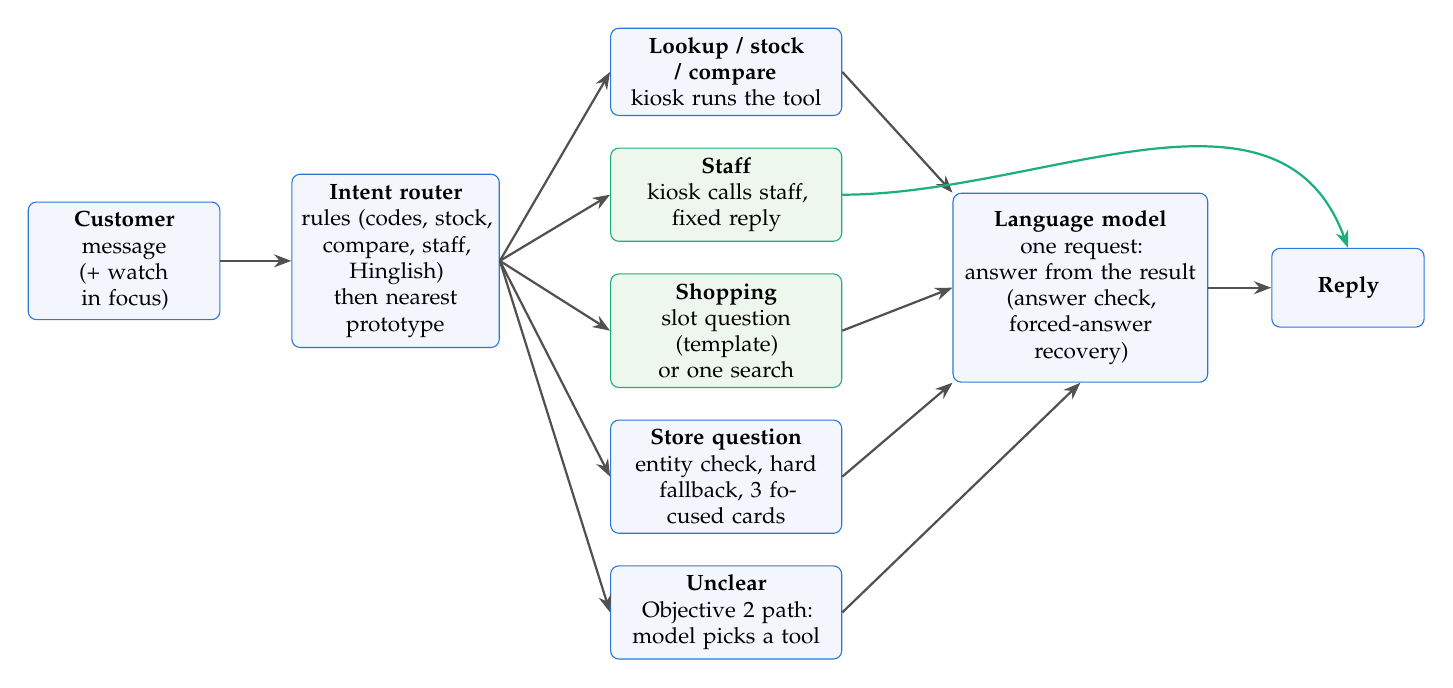
\begin{tikzpicture}[
  node distance=4mm and 7mm,
  box/.style={draw=qblue, fill=boxfill, rounded corners=3pt, align=center, font=\footnotesize, minimum height=10mm,
              text width=27mm},
  fix/.style={draw=qaqua, fill=fixfill, rounded corners=3pt, align=center, font=\footnotesize, minimum height=10mm,
              text width=27mm},
  arr/.style={-{Stealth[length=2.2mm]}, thick, ink2}]
\node[box, text width=22mm] (msg) {\textbf{Customer}\\message (+ watch\\in focus)};
\node[box, right=9mm of msg, text width=24mm, minimum height=22mm] (rt) {\textbf{Intent router}\\rules (codes, stock,\\compare, staff,
Hinglish)\\then nearest\\prototype};
\node[box, right=14mm of rt, yshift=24mm] (h) {\textbf{Lookup / stock / compare}\\kiosk runs the tool};
\node[fix, below=of h] (st) {\textbf{Staff}\\kiosk calls staff,\\fixed reply};
\node[fix, below=of st] (sh) {\textbf{Shopping}\\slot question (template)\\or one search};
\node[box, below=of sh] (kn) {\textbf{Store question}\\entity check, hard\\fallback, 3 focused cards};
\node[box, below=of kn] (un) {\textbf{Unclear}\\Objective~2 path:\\model picks a tool};
\node[box, right=14mm of kn, yshift=24mm, text width=30mm, minimum height=24mm] (llm) {\textbf{Language model}\\one request:\\answer from the result\\
(answer check,\\forced-answer recovery)};
\node[box, right=8mm of llm, text width=17mm] (out) {\textbf{Reply}};
\draw[arr] (msg) -- (rt);
\foreach \n in {h,st,sh,kn,un} { \draw[arr] (rt.east) -- (\n.west); }
\draw[arr] (h.east) -- (llm.north west);
\draw[arr] (kn.east) -- (llm.south west);
\draw[arr] (un.east) -- (llm.south);
\draw[arr] (sh.east) -- (llm.west);
\draw[arr] (llm) -- (out);
\draw[arr, qaqua] (st.east) to[out=0, in=110] (out.north);
\end{tikzpicture}}
\caption{One turn in O3-final. Green: no model call (a template, a fixed reply or the kiosk's own staff call; a
shopping turn calls the model only to present the search results). Blue: the model answers from one compact result.
The entity check (other brands, smartwatches, designs that do not exist) and the hard fallback reply without the model
too.}
\label{fig:pipeline}
\end{figure}

The hardware is unchanged: an Intel Core i5-1240P laptop with 16\,GB of RAM and Intel Iris Xe graphics stands in for both
tiers. The 2B runs on four CPU threads (Tier A), the 4B on the integrated GPU through Vulkan (Tier B), both in llama.cpp's
\texttt{llama-server}~\cite{llamacpp}. Retrieval runs in the assistant's process: BM25~\cite{bm25} and
bge-small~\cite{bge} fused and re-ranked by a MiniLM cross-encoder~\cite{minilm}, now on the OpenVINO runtime with an
8-bit re-ranker and no PyTorch.

% ===========================================================================
\section{Method}\label{sec:method}
% ===========================================================================

\subsection{Protocol}
Every change was tuned on development data only, kept or dropped by a rule written in the project's objectives document
before its run, and confirmed once on the fresh test set. A keep rule compares the new configuration with the previous
one on the same dev cases, per model. A set is ``better'' or ``worse'' only if the paired bootstrap 95\%
interval~\cite{efron} excludes zero \emph{and} the difference exceeds a noise bound measured from repeated greedy runs
(identical runs changed 0--2.8\% of outcomes); otherwise it is a tie. Paired right/wrong outcomes also get an exact
McNemar test~\cite{mcnemar}. Where a result was read after the fact, or a rule was not followed to the letter, the
deviation is stated where it happened (Table~\ref{tab:steps} and Section~\ref{sec:decisions}).

\paragraph{Data.} The development sets are those of Objective~2 (the dev split of the store-question set, the v1.1
tool cases rebuilt as v1.2) plus new material: 60 dev follow-up questions and 40 dev shopping dialogues, played by a
rule-based customer simulator with hidden profiles (recipient, budget, occasion, strap, size), so that dialogues need
no second model. Every automatic check is the Objective~2 scorer, with three phrasing fixes made in Step~13 and applied
to both sides of every later comparison.

\paragraph{Runs and machines.} Quality runs used the laptop's GPU for both models; timing that decides anything was
measured in place on the laptop (CPU for Tier~A). From Step~9, CPU-only work could run in a private cloud notebook;
those runs record their machine, and no latency from another machine is compared with the laptop's.

\paragraph{Software.} The harness, scorers and analysis scripts were written for this project. An AI coding assistant
helped write and debug parts of this code.

\subsection{Development steps}
Table~\ref{tab:steps} summarises the thirteen development steps. The text below highlights what each step taught.

{\small
\begin{xltabular}{\textwidth}{>{\raggedright\arraybackslash}p{2.9cm} >{\raggedright\arraybackslash}p{4.4cm} L}
\caption{Development steps, their keep rules in brief, and their outcomes on dev.}\label{tab:steps}\\
\toprule
Step & Change & Outcome on dev \\
\midrule
\endfirsthead
\toprule Step & Change & Outcome on dev \\ \midrule \endhead
1 Baseline & Freeze O3-B0; log rounds, tokens read and written per round, first-word time & All checks pass (0
errors, cache misses 0\%, first-word formula within 3--11\%). Tier~A first word 14.0\,s (store) and 12.8\,s (tools);
the 2B averages 2.5--2.65 rounds and hits the round limit on 30\% of store questions. \\
2 Data and scorer fixes & Label fixes, ``watch'' no longer matching every product, wider search description,
shown-card credit & Kept (all ties; 2B answerable $-8.3$ traced to loops, handled in Step~3). \\
3 Tool output v2, loop guard & One line per result, 3 results, ``not listed'' for missing fields, repeated calls
answered ``already shown'', last round without tools & Kept, with a disclosed deviation: tokens per tool output fell
46--49\% on store questions against a 50\% rule. 2B store questions +12.6 [+5.2, +20.0]; round-limit hits 33 $\to$
0. \\
4 Intent router & Rules, then the nearest of 7 route prototypes (bge-small); low margin $\to$ unclear & Kept. 97.2\%
route accuracy, 2.1\% of store questions misrouted, 0.2\,ms. Tool cases now tie with no retrieval: the Objective~2
regression is gone. Hinglish tool cases 33\% $\to$ 89\% (2B). \\
5 Kiosk-run tools & The kiosk runs lookup, stock, compare and staff from the message; one model request & Kiosk-run
tools kept; one-request store answers dropped (2B store questions 62\% $\to$ 27\%). Hand-offs 17\% $\to$ 100\% (2B). \\
6 Guided discovery & Slot extractor; at most 2 template questions, then one search & Kept after two fix rounds (the
fixes came from dev dialogues, so the test set decides). Fit 100\%, 1.0 model request per dialogue; kiosk time
33.6 $\to$ 9.9\,s (2B). One condition failed (4B shopping cases), carried to Step~7. \\
7 Forced answers, prompt v1.2 & 7a: a printed tool call is recovered or replaced; 7: new prompt and staff rules & 7a
kept (closes Step~6's failure; no printed call reaches a customer). Prompt v1.2 not kept: staff calls on answerable
questions did not fall and two 4B subsets fell. \\
8 Knowledge path & Entity check and hard fallback (no model call); a staff check before a ``can't answer'' hand-off &
Kept with a disclosed deviation: unanswerable +5.1 for both models, a tie where ``better'' was required; no subset
worse. \\
9 Re-ranker trial & A fine-tuned MiniLM and a multilingual re-ranker & Not kept: none met the 300\,ms cap; halving the
re-rank depth costs 5.6--7.2 points of Recall@3. \\
10 Cited answers & Check every number and spec in an answer against what was shown & The check against everything shown
kept (unsupported replies 6.9\% $\to$ 3.1\%, 4B; no correct answer lost). Citation by card number dropped ($-47$ to
$-53$ points). \\
11 Follow-up retrieval & Previous turn and the watch in focus added to the query; focus card first & Kept after one fix
(store topics are new questions): follow-ups +33.3 (4B) and +15.0 (2B), no topic switch lost. \\
12 Retrieval speed & OpenVINO runtime without PyTorch, static 8-bit re-ranker & Kept: 230\,ms median (was 463--532),
+638\,MB, recall unchanged. \\
13 Generation speed & Focused cards, short replies, two tool calls per round; speculative decoding trial & 2B: all
three kept (total reply $-2.1$\,s on store questions in place). 4B: the short-reply rule made it print tool calls, so it
keeps focused cards and parallel calls only. Speculative decoding: none qualified. \\
\bottomrule
\end{xltabular}}

\paragraph{What the steps showed.} Three lessons recur. First, \textbf{the small model's loops, not its knowledge, cost
the most}: in Steps~2--3, 9 of the 11 store questions the 2B lost were empty replies at the round limit, and a guard that
answers a repeated call with ``already shown'' fixed them. Second, \textbf{moving work out of the model pays twice}: the
router and kiosk-run tools removed the tool-case regression of Objective~2 and the slowest waits at once, because a tool
call written by the model is both the slowest part of a turn and the most error-prone. Third, \textbf{a stricter output
format can backfire}: the 4B printed tool calls as text when its replies were capped in length (Step~13), and the
citation format cost half of all correct answers because the models seldom cited (Step~10).

\paragraph{Speculative decoding (Step 13b).} Drafting from n-grams, from a 0.8B draft model, and from the models' own
multi-token-prediction layers was trialled with a rule fixed in advance: replies identical to plain decoding as often as
plain decoding agrees with itself, and at least 1.2$\times$ faster writing. On four CPU threads nothing wrote faster than
1.02$\times$. On the GPU the 4B's prediction layers wrote 1.29$\times$ faster, but the only file that contains them is a
different quantisation (25 of 70 replies identical to the deployed file), so it was excluded because the models are fixed.

\subsection{The test set and the confirming run (Step 14)}
O3-T was built once, before any Step~14 run, with new seeds: 192 tool cases (117 freshly generated, plus the held-out
halves of the discovery and Hinglish categories), 463 store questions (311 fresh plus held-out hand-written types), the
60 test follow-ups set aside in Step~11, and 60 fresh dialogue profiles. Hinglish appears in every set (37 tool cases,
63 store questions, 26 follow-ups, 18 dialogues). Objective~3 had never run a test case.

The rules, fixed before the runs, were, for each tier and O3-final against O3-B0: (1) no primary set is worse; (2)
follow-ups are better; (3) the dialogues meet the Step~6 targets with fit not lower; (4) Tier~A only, in place on CPU,
the median total reply time falls and the first word is not later. The primary family (store questions, tool cases and
follow-ups on both tiers, six tests) is Holm-adjusted~\cite{holm}. A tier is confirmed if all its rules hold.

\subsection{Ablation, judging and scorecard (Step 15)}
\paragraph{The ladder.} Each rung adds the changes kept on dev, in the order they were kept: O3-B0; R1 tool output and
loop guard; R2 router; R3 kiosk-run tools, discovery and forced-answer recovery; R4 fallback, entity and staff checks;
R5 answer check and follow-up retrieval; R6 = O3-final (speed work). A variant without the router measures its own
effect. Two references serve two criteria: oracle cards on store questions, and no retrieval on tool cases. Each rung
copies the settings of the dev run that kept it, and the rebuilt O3-B0 and O3-final were checked to equal the Step~14
settings. The ladder ran on cloud T4 GPUs with one llama.cpp build compiled for that card, so every rung shares a
machine and a build; it is descriptive (no adjustment), since the confirming decision was Step~14's. It first ran on
cloud CPUs and was moved to the GPU, before any GPU run, because it would have taken about five days; the finished CPU
runs became a cross-check.

\paragraph{The judge.} Hallucination, false refusals and unsupported details cannot be checked automatically, so they
were judged blind, with Objective~2's protocol and instructions (Appendix~\ref{app:judge}). The packet held 829 replies
from the Step~14 runs of O3-final and O3-B0, both models: every unanswerable and near-miss question, 60 answerable
questions sampled by type (the same in every run), and every other answerable reply that looked like a refusal. Model,
configuration and run were hidden and the order shuffled. Labelling was done by a large general-purpose language model
from a different model family than either candidate~\cite{llmjudge}, run as seven independent instances of about 120
items each, without access to the key. A consistency pass then set 8 labels from ``unsupported'' to ``declined'': five
pairs of identical items had received different labels, all on replies that only say the store does not sell an item or
brand, which the instructions count as a decline. The author labelled 50 random items without seeing the judge's labels.
113 empty replies were labelled automatically as declined.

\paragraph{Statistics.} Rates carry Wilson 95\% intervals~\cite{wilson}; Cohen's $\kappa$~\cite{kappa} measures
judge--human agreement.

% ===========================================================================
\section{Results}\label{sec:results}
% ===========================================================================

\subsection{The confirming run (Step 14)}
Figure~\ref{fig:step14} and Table~\ref{tab:step14} give the confirming run. On the 2B, O3-final is better on store
questions (+17.7 points) and tool cases (+15.1); on the 4B, follow-ups rise from 66.7\% to 90.0\% (+23.3). No primary
set is worse on either tier.

\begin{figure}[H]
\centering
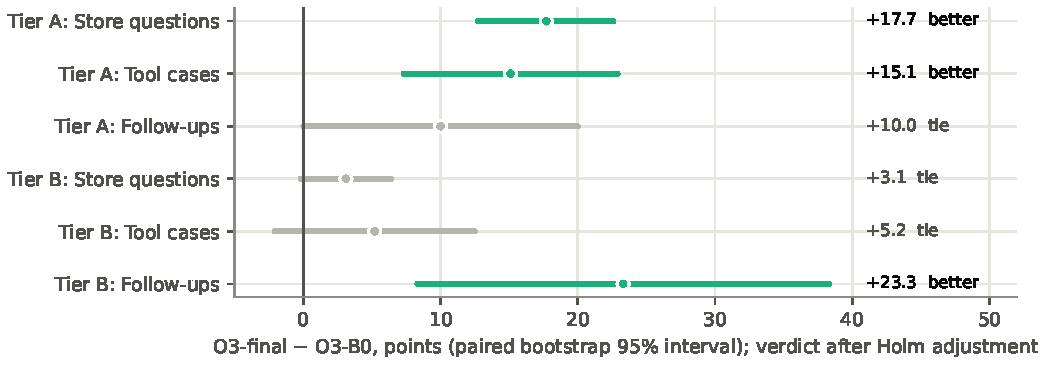
\includegraphics[width=0.92\textwidth]{figs/fig_step14.pdf}
\caption{O3-final against O3-B0 on the test set, paired. Green: better after the Holm adjustment across the six primary
tests.}
\label{fig:step14}
\end{figure}

\begin{table}[H]
\centering\small
\caption{Primary family on O3-T (Holm-adjusted across six tests).}\label{tab:step14}
\begin{tabular}{llrrrlrl}
\toprule
Tier & Set & Cases & O3-B0 & O3-final & Difference [95\% CI] & Holm $p$ & Verdict \\
\midrule
A & Store questions & 424 & 51.9\% & 69.6\% & +17.7 [+12.7, +22.6] & $<10^{-10}$ & better \\
A & Tool cases & 192 & 62.5\% & 77.6\% & +15.1 [+7.3, +22.9] & 0.002 & better \\
A & Follow-ups & 60 & 80.0\% & 90.0\% & +10.0 [0.0, +20.0] & 0.276 & tie \\
B & Store questions & 424 & 78.3\% & 81.4\% & +3.1 [$-$0.2, +6.4] & 0.276 & tie \\
B & Tool cases & 192 & 78.1\% & 83.3\% & +5.2 [$-$2.1, +12.5] & 0.276 & tie \\
B & Follow-ups & 60 & 66.7\% & 90.0\% & +23.3 [+8.3, +38.3] & 0.026 & better \\
\bottomrule
\end{tabular}
\end{table}

\paragraph{Verdicts.} \textbf{Tier~B is confirmed}: no set is worse, follow-ups are better, and the dialogues meet every
target. \textbf{Tier~A is not confirmed, on rule (2) alone}: its follow-ups rose from 80\% to 90\% (2 lost, 8 gained),
which is a tie after the adjustment. O3-B0 already answered 80\% of the 2B's test follow-ups (71.7\% on dev), so there
was little room for the gain the rule asked for; the miss stands. Every other Tier~A rule holds, including the timing
rule (Section~\ref{sec:speed}).

\paragraph{Reported, not deciding.} On unanswerable and near-miss questions, the automatic check (a correct decline
counts) is better for the 2B (33.1\% $\to$ 54.0\%, +20.9 [+12.9, +28.8]) and ties for the 4B (+2.9 [$-$4.3, +10.1]). By
origin, the 2B's gains hold on both fresh and held-out questions; the 4B's store questions improve on fresh questions
(+5.9) and tie on held-out ones. Hinglish store questions tie for both models (2B 50.0\% $\to$ 50.0\%; 4B 58.1\% $\to$
54.8\%). Two 4B subsets fell: hand-offs (92.9\% $\to$ 64.3\%, 4 of 14 lost) and topic-switch follow-ups (100\% $\to$
60\%); Section~\ref{sec:failures} traces both. The pre-registered prompt v1.2 candidate for Tier~A was better on store
questions (+4.2 [+1.2, +7.5]) and tied elsewhere; it is not adopted, because choosing a configuration on the test set
would spend it.

\paragraph{Dialogues.} Figure~\ref{fig:dialogues} shows the 60 fresh shopping dialogues. O3-final reaches a
recommendation in every dialogue, always knows at least two of the four slots first, asks at most two questions, and
shows watches that fit what the customer said 97\% of the time on both models (O3-B0: 87\% and 63\%). It needs one
model request per dialogue instead of 3.6--4.0, and the time at the kiosk falls from 25.6 to 9.7\,s (2B) and from 59.5
to 17.6\,s (4B).

\begin{figure}[H]
\centering
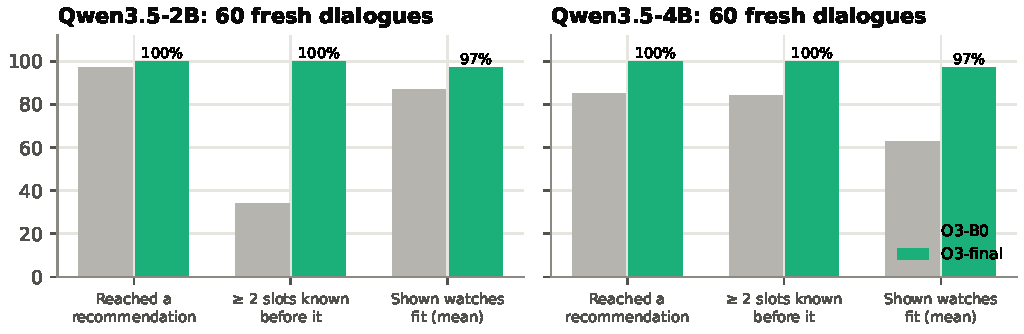
\includegraphics[width=0.9\textwidth]{figs/fig_dialogues.pdf}
\caption{Simulated shopping dialogues on the test profiles. Fit: share of shown watches that meet every constraint the
customer had stated.}
\label{fig:dialogues}
\end{figure}

\subsection{The ablation ladder (Step 15)}\label{sec:ladder}
Figure~\ref{fig:ladder} and Table~\ref{tab:ladder} attribute the gains. Each cell is a pass rate on the test set, with
the step from the rung below.

\begin{figure}[H]
\centering
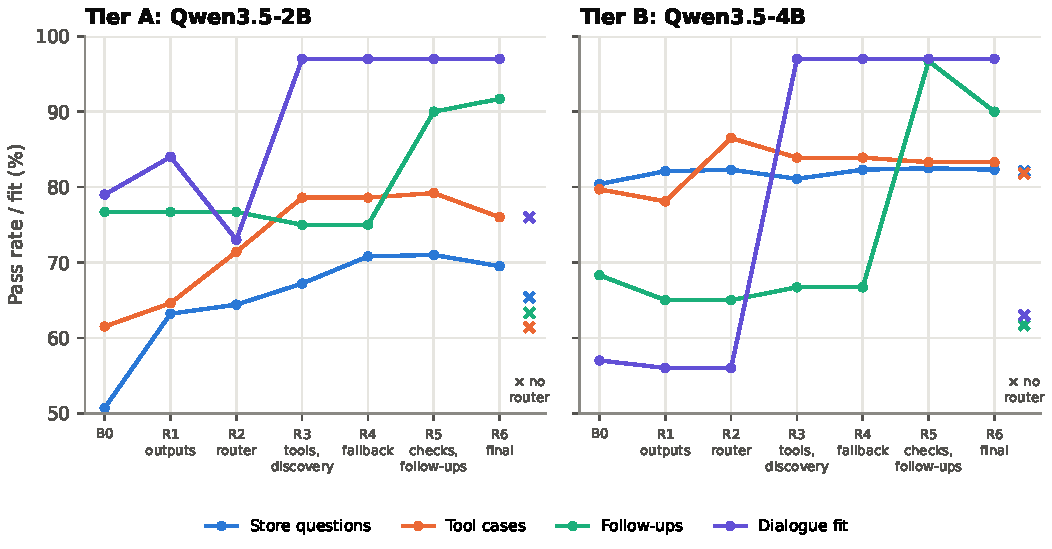
\includegraphics[width=\textwidth]{figs/fig_ladder.pdf}
\caption{The cumulative ladder on O3-T (cloud T4 GPU, one build). Crosses: O3-final without the router.}
\label{fig:ladder}
\end{figure}

{\small
\begin{table}[H]
\centering
\caption{The ladder on O3-T. Steps from the rung above in points; $\blacktriangle$/$\blacktriangledown$ better/worse
by the dev rule (noise bound and interval), unadjusted.}\label{tab:ladder}
\resizebox{\textwidth}{!}{%
\begin{tabular}{lllllll}
\toprule
& \multicolumn{3}{c}{Tier A (2B)} & \multicolumn{3}{c}{Tier B (4B)} \\
\cmidrule(lr){2-4}\cmidrule(lr){5-7}
Rung & Store questions & Tool cases & Follow-ups & Store questions & Tool cases & Follow-ups \\
\midrule
O3-B0 & 50.7 & 61.5 & 76.7 & 80.4 & 79.7 & 68.3 \\
R1 tool output, loop guard & 63.2 (+12.5\,$\blacktriangle$) & 64.6 (+3.1) & 76.7 (0.0) & 82.1 (+1.7) & 78.1 ($-$1.6) & 65.0 ($-$3.3) \\
R2 router & 64.4 (+1.2) & 71.4 (+6.8\,$\blacktriangle$) & 76.7 (0.0) & 82.3 (+0.2) & 86.5 (+8.3\,$\blacktriangle$) & 65.0 (0.0) \\
R3 kiosk tools, discovery & 67.2 (+2.8\,$\blacktriangle$) & 78.6 (+7.3) & 75.0 ($-$1.7) & 81.1 ($-$1.2) & 83.9 ($-$2.6) & 66.7 (+1.7) \\
R4 fallback, entity, staff & 70.8 (+3.5\,$\blacktriangle$) & 78.6 (0.0) & 75.0 (0.0) & 82.3 (+1.2) & 83.9 (0.0) & 66.7 (0.0) \\
R5 answer check, follow-ups & 71.0 (+0.2) & 79.2 (+0.5) & 90.0 (+15.0\,$\blacktriangle$) & 82.5 (+0.2) & 83.3 ($-$0.5) & 96.7 (+30.0\,$\blacktriangle$) \\
R6 = O3-final (speed) & 69.5 ($-$1.4) & 76.0 ($-$3.1) & 91.7 (+1.7) & 82.3 ($-$0.2) & 83.3 (0.0) & 90.0 ($-$6.7\,$\blacktriangledown$) \\
\midrule
O3-final without router & 65.4 & 61.4 & 63.3 & 82.1 & 81.8 & 61.7 \\
\bottomrule
\end{tabular}}
\end{table}}

\begin{itemize}
  \item \textbf{The 2B's store questions gain most from the loop guard} (R1, +12.5; answerable questions +18.6): empty
        replies at the round limit fell from 108 to 39. The fallback and entity check (R4) add +10.8 on unanswerable
        and near-miss questions.
  \item \textbf{Tool cases gain from the router and the kiosk-run tools} (R2 and R3, +14.0 together on the 2B; R2 +8.3
        on the 4B). Without the router, the 2B's tool cases fall back to O3-B0's level (61.4\%).
  \item \textbf{Follow-ups gain at R5}, where retrieval keeps the watch in focus: +15.0 (2B) and +30.0 (4B).
  \item \textbf{Dialogues gain at R3}, where discovery starts: fit +23.7 (2B) and +41.7 (4B). The same rung costs the
        4B 3.6 points on unanswerable and near-miss questions, which R4's fallback and entity check win back (+5.8).
  \item \textbf{The speed work (R6) costs a little quality}: 2B tool cases $-$3.1 and the 4B's follow-ups $-$6.7, the
        latter in topic-switch follow-ups like the store-hours losses of Section~\ref{sec:failures}. Nothing at R6 is
        worse for the 2B by the rule.
  \item \textbf{The router's own effect} (O3-final against O3-final without it) is large on the 2B: store questions +3.4,
        unanswerable +10.8, tool cases +14.3, follow-ups +28.3 and dialogue fit +21.4, all better. On the 4B it matters
        for follow-ups (+28.3) and dialogue fit (+34.6) but not for single questions, which the 4B handles on the
        always-retrieve path.
\end{itemize}

Figure~\ref{fig:reading} shows why the turns got faster. Tokens read before the answer fell from 852 to 427 (2B store
questions) and from 1,066 to 259 (2B tool cases); model requests per tool case fell from 2.8 to 1.0, almost entirely at
R2--R3, where the model stops writing tool calls.

\begin{figure}[H]
\centering
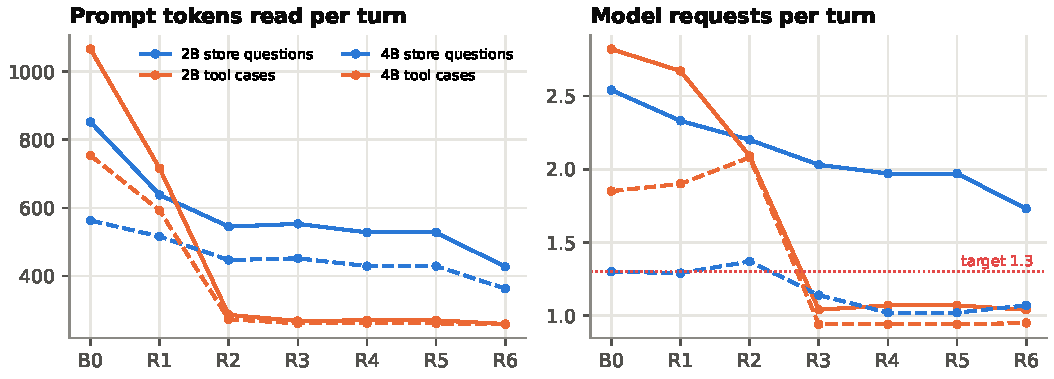
\includegraphics[width=0.95\textwidth]{figs/fig_reading.pdf}
\caption{Reading per turn along the ladder. Solid: 2B; dashed: 4B.}
\label{fig:reading}
\end{figure}

\paragraph{The machines agree.} O3-B0 and O3-final were run on three set-ups: the laptop (Step~14), cloud CPUs and cloud
GPUs. Of the 40 paired comparisons with the laptop, 38 are ties; the two exceptions are the 4B's O3-B0 on answerable
questions (+5.3 points on the GPU and +3.5 on the CPU over the laptop). All 20 comparisons between the cloud CPU and the
cloud GPU are ties. The ladder therefore
speaks for the deployed runs. In the no-router variant, 14 of the 2B's cases (11 store questions, 3 tool cases) failed
every time: llama-server could not parse the 2B's tool call because the 120-token reply cap cut it off. These cases are
left out of that variant's comparisons.

\subsection{Hallucination, refusals and unsupported details (judged)}\label{sec:judged}
Figure~\ref{fig:judged} and Table~\ref{tab:judged} give the judged rates on the Step~14 replies.

\begin{figure}[H]
\centering
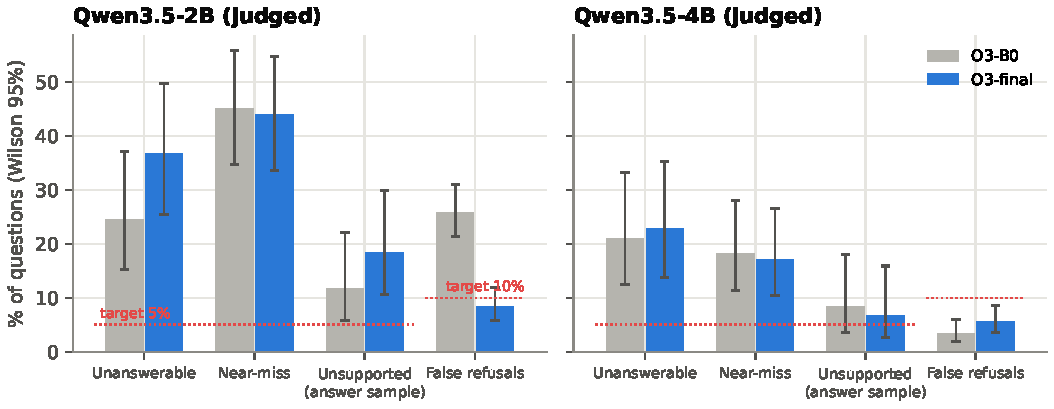
\includegraphics[width=0.95\textwidth]{figs/fig_judged.pdf}
\caption{Judged rates, O3-B0 against O3-final (Wilson 95\% intervals). Dotted: the targets.}
\label{fig:judged}
\end{figure}

\begin{table}[H]
\centering\small
\caption{Judged rates on O3-T.}\label{tab:judged}
\resizebox{\textwidth}{!}{%
\begin{tabular}{llrrrrr}
\toprule
Model & Configuration & Unanswerable & Near-miss & Hinglish (both) & Unsupported (sample) & False refusals \\
\midrule
2B & O3-B0 & 24.6\% & 45.1\% & 25.0\% & 11.7\% & 25.9\% \\
2B & O3-final & 36.8\% & 43.9\% & 62.5\% & 18.3\% & 8.3\% \\
4B & O3-B0 & 21.1\% & 18.3\% & 25.0\% & 8.3\% & 3.4\% \\
4B & O3-final & 22.8\% & 17.1\% & 29.2\% & 6.7\% & 5.6\% \\
\midrule
\multicolumn{2}{l}{Questions} & 57 & 82 & 24 & 60 & 324 \\
\bottomrule
\end{tabular}}
\end{table}

\begin{itemize}
  \item \textbf{Hallucination is not reduced.} O3-final ties O3-B0 on every judged hallucination measure for both models
        (paired changes from $-$1.2 to +12.3 points, all intervals including zero). Both models stay far above the 5\%
        target: 23\% and 17\% (4B), 37\% and 44\% (2B), on unanswerable and near-miss questions.
  \item \textbf{The 2B traded refusals for answers.} Its false refusals fell from 25.9\% to 8.3\%, now within target,
        because the loop guard turned empty replies at the round limit into answers. On answerable questions that is a
        gain; on unanswerable ones some of the same replies now carry claims, and its unanswerable rate rose from 24.6\%
        to 36.8\% (+12.3 [$-$1.8, +28.1], a tie). Its Hinglish replies are the weakest: 15 of 24 unsupported.
  \item \textbf{Where the claims come from.} ``Negative'' questions (asking whether a design has a feature it lacks)
        and missing attributes account for 32 of the 2B's 57 unsupported replies; typical errors are a ``no'' for a
        whole collection inferred from three cards, an incomplete colour list, water-resistance advice (``30\,m is safe
        for the shower''), and a ``yes'' to a service the store does not offer. Designs that do not exist produced no
        unsupported reply for either model: the entity check answers them without the model.
  \item \textbf{Two measures of unsupported details disagree.} The automatic check (a number, code or spec word found
        in neither the gold card nor the tool results) finds 2.9\% (2B) and 4.9\% (4B), within target; the judge finds
        18.3\% and 6.7\% in a sample of 60 answers. The automatic check only sees checkable details; the judge also
        counts wrong ``yes'' and ``no'' answers and claims without numbers.
\end{itemize}

\paragraph{Agreement with the human check.} On 49 random items (one left unlabelled), the author and the judge agreed
exactly on 59\% ($\kappa = 0.38$) and on 40 of 49 (82\%) for ``unsupported or not''. Every disagreement went the same way:
whenever the author marked a reply unsupported or declined, the judge agreed; the judge called 9 replies unsupported and
11 declined that the author accepted. The 11 are mostly ``not listed'' and ``staff are coming'' replies, which do not
affect hallucination; several of the 9 are genuine errors on reading (a ``yes, it has a purple dial'' followed by a
royal-blue watch). This is the pattern of Objective~2 ($\kappa = 0.34$), so the judged hallucination rates are again
upper estimates; even so, the 4B's 23\% would reach 5\% only if four in five flagged replies were false alarms.

\subsection{Speed and memory}\label{sec:speed}
Figure~\ref{fig:wait} gives the Tier~A timing rule, measured in place on the laptop CPU (70 test cases, two
alternating repeats). The median total reply time fell by 4.4\,s on store questions and 22.3\,s on tool cases, and the
first word came 3.9\,s and 19.1\,s sooner: rule (4) holds.

\begin{figure}[H]
\centering
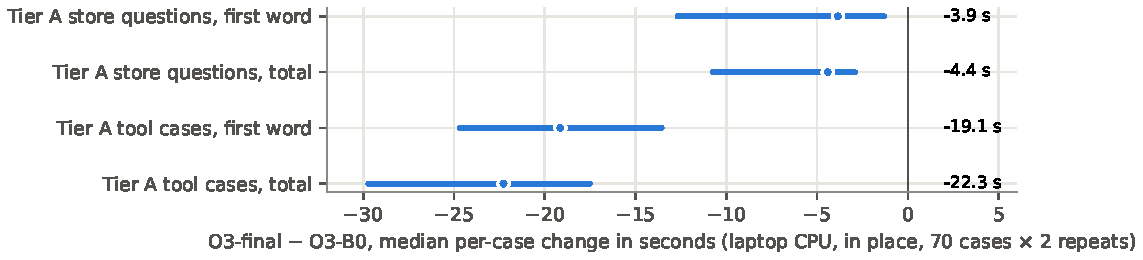
\includegraphics[width=0.92\textwidth]{figs/fig_wait.pdf}
\caption{Tier A in place: median per-case change, O3-final $-$ O3-B0, with bootstrap 95\% intervals over cases.}
\label{fig:wait}
\end{figure}

In absolute terms, Tier~A's first word now comes after 4.6\,s at the median but 15.5\,s at the 90th percentile, and a
full reply takes 10.1\,s. The tail is the store questions that still take several model rounds (1.73 per turn). Tier~B
on the integrated GPU reaches the first word in 3.9\,s at the median (90th percentile 14.5\,s) and the full reply in
11.9\,s, with 1.03 rounds per turn. Retrieval takes 286\,ms at the median in place. Peak memory is 4.04\,GB (Tier~A) and
5.70\,GB (Tier~B), within the 5 and 10\,GB budgets; the 8-bit retrieval stack uses 0.29\,GB more than O3-B0's on
Tier~A, within the 0.8\,GB allowance.

\subsection{Scorecard}\label{sec:scorecard}
Table~\ref{tab:score} sets O3-final against every criterion. Fourteen of 24 decided criteria are met for Tier~A and 13
of 23 for Tier~B. One criterion cannot be measured on O3-final: the router leaves only one test tool case to the model.

{\small
\begin{xltabular}{\textwidth}{>{\raggedright\arraybackslash}p{5.6cm} >{\raggedright\arraybackslash}p{2.2cm}
>{\raggedright\arraybackslash}p{2.6cm} >{\raggedright\arraybackslash}p{2.6cm} L}
\caption{Scorecard: O3-final on O3-T.}\label{tab:score}\\
\toprule
Criterion & Target & Tier A (2B) & Tier B (4B) & \\
\midrule
\endfirsthead
\toprule Criterion & Target & Tier A (2B) & Tier B (4B) & \\ \midrule \endhead
Right tool, valid arguments (system) & $\ge 90\%$ & 77.6\% \missed & 83.3\% \missed & \\
Right tool, model alone & $\ge 80\%$ & 1 case \na & 1 case \na & \\
Valid arguments, model calls & $\ge 98\%$ & 100\% \met & 100\% \met & \\
Router accuracy & $\ge 95\%$ & 94.7\% \missed & 94.7\% \missed & \\
Store questions sent to a tool path & $\le 3\%$ & 3.6\% \missed & 3.6\% \missed & \\
Slots known before recommending & $\ge 85\%$ & 100\% \met & 100\% \met & \\
Questions before recommending & $\le 2$ & max 2 \met & max 2 \met & \\
Recommendations fit & $\ge 90\%$ & 97\% \met & 97\% \met & \\
Staff called when needed & $\ge 90\%$ & 64\% \missed & 64\% \missed & \\
Unneeded staff calls & $\le 5\%$ & 10.2\% \missed & 0.9\% \met & \\
Staff tickets per turn & $\le 1$ & 0 over \met & 0 over \met & \\
No tool-case regression & not below & +0.0 \met & $-$4.7 (tie) \met & \\
Answerable vs oracle & $\ge -5$ pts & +5.6 \met & $-$3.9 \met & \\
Hallucination, unanswerable & $\le 5\%$ & 36.8\% \missed & 22.8\% \missed & \\
Hallucination, near-miss & $\le 5\%$ & 43.9\% \missed & 17.1\% \missed & \\
False refusals & $\le 10\%$ & 8.3\% \met & 5.6\% \met & \\
Unsupported details (automatic) & $\le 5\%$ & 2.9\% \met & 4.9\% \met & \\
Unsupported details (judged sample) & $\le 5\%$ & 18.3\% \missed & 6.7\% \missed & \\
First word, median / p90 & see Table~\ref{tab:criteria} & 4.6 / 15.5\,s \missed & 3.9 / 14.5\,s \missed & \\
Full reply, median & $\le 11$\,s & 10.1\,s \met & 11.9\,s \missed & \\
Model rounds per turn & $\le 1.3$ & 1.62 \missed & 1.03 \met & \\
Tokens read vs O3-B0 & $\le 50\%$ & 43\% \met & 57\% \missed & \\
Retrieval latency, median & $\le 300$\,ms & 286\,ms \met & -- & \\
Peak memory & 5 / 10\,GB & 4.04\,GB \met & 5.70\,GB \met & \\
Memory added & $\le 0.8$\,GB & +0.29\,GB \met & $-$0.34\,GB \met & \\
\bottomrule
\end{xltabular}}

\noindent Against Objective~2, the regression on tool cases is gone, false refusals are within target for both models,
the dialogue targets are met, and retrieval latency and memory now meet their targets. The tool, router, staff and
hallucination targets are missed, and the first-word target is met at the median but not in the tail.

\subsection{Failure analysis: what the test set exposed}\label{sec:failures}
A case review of every changed test case found five patterns. They were found on the test set, so Objective~3 does not
fix them; they are handed to Objective~4 with its own fresh test set.
\begin{enumerate}
  \item \textbf{Try-on requests with a product code go to lookup.} ``Could I wear 3294AL02 for a minute?'' and
        ``1479PF01 pehen ke dekhna chahta hoon'' are routed to the product lookup, so the kiosk shows the watch instead
        of calling staff; the 4B then prints a staff call that the forced-answer rule cannot run, and the customer sees
        the empty-reply line (6 tool cases for the 4B, 3 for the 2B). This is most of the 4B's hand-off drop.
  \item \textbf{``Can I buy X today?'' skips the stock check.} The staff route calls staff for a purchase without
        checking stock, and one of the three watches was out of stock.
  \item \textbf{The slot extractor misses words seen only on the test set.} It drops the customer's gender (``I'm a
        man'', ``Woman, any budget''; 5 cases each) and, for the 4B, Hinglish budgets worded ``3000 ke andar'' (3) and
        one in-stock-only request. Like the router and the policy check in Steps~4 and~6, rules tuned on dev overfit.
  \item \textbf{Store hours after a watch.} ``Store kab tak khula hai?'' and ``What are your store hours?'' after a
        product get a reply saying the hours were not shown (4B: 4 of its topic-switch losses). This topic switch had
        flipped between dev runs before (Step~12).
  \item \textbf{Short replies cut spec answers on the 2B.} Its 120-token cap cut five specification answers before the
        asked fact; the same cap truncated the tool calls that failed in the no-router variant.
\end{enumerate}
Beyond these, the judged errors in Section~\ref{sec:judged} are behaviours of the model given correct information:
inferring a collection-wide ``no'' from a few cards, completing lists from memory, and adding advice. Retrieval and
routing cannot fix these; training can.

% ===========================================================================
\section{Decisions and reasoning}\label{sec:decisions}
% ===========================================================================
{\small
\begin{xltabular}{\textwidth}{>{\raggedright\arraybackslash}p{3.6cm} >{\raggedright\arraybackslash}p{4.4cm} L}
\caption{Decision log.}\label{tab:decisions}\\
\toprule
Decision & Evidence & Reasoning \\
\midrule
\endfirsthead
\toprule Decision & Evidence & Reasoning \\ \midrule \endhead
Keep both models fixed & Objective~1 selected them; Objective~4 fine-tunes them & Changes to the pipeline are then the
only cause of any difference. \\
Rule per step, written before its run & Many small changes, each tempting to keep & A result read after the fact cannot
move its own threshold; deviations are named instead. \\
Noise bound with the interval & Greedy repeats flip 0--2.8\% of outcomes & A difference smaller than the system's own
noise is not evidence. \\
Keep Step~3's compact view despite 46--49\% (rule: 50\%) & It added quality and halved reading on tool cases &
Disclosed as a deviation; the ladder shows R1 is the 2B's largest single gain. \\
Router with a margin, not rules alone & Rules alone: 97\% dev, 90\% on the old test split & Rules overfit; a low-margin
message keeps the Objective~2 path rather than a wrong one. \\
Kiosk-run tools, not one-request store answers & One-request answers: 2B 62\% $\to$ 27\% & The 2B printed its tool call
as text when tools were off; the fallback in the rule applied. \\
Templates for slot questions & Blind rubric: 4.9 vs 2.9 (2B) & Templates are clearer, instant and need no model
call. \\
Drop prompt v1.2; test it only as a candidate & Its gain was seen on dev after the fact & Pre-registered for the test
split, reported, not adopted. \\
Keep Step~8 with a tie on unanswerable & +5.1 for both, ``better'' required & Disclosed; nothing worse, and Step~14
checked it on 139 test questions. \\
Answer check against everything shown, not citations & Citations: $-47$ to $-53$ points & The models seldom cited; a
strict format destroyed correct answers. \\
Static 8-bit re-ranker & 230\,ms vs 463--532\,ms, recall unchanged & Meets both targets; thresholds re-derived by their
own rules. \\
4B without the short-reply rule & It printed tool calls with it (14 on dev) & The leave-one-out runs located the
cause. \\
No speculative decoding & Nothing qualified; the only fast option needs another model file & The models are fixed. \\
Do not fix test-set failures in Objective~3 & Found on O3-T & Fixing them would tune on the test set; Objective~4 has
its own. \\
Move the ladder to the GPU & CPU ladder projected at five days & Changed before any GPU run; the CPU runs became a
cross-check, and the machines agree. \\
\bottomrule
\end{xltabular}}

% ===========================================================================
\section{Limitations and threats to validity}\label{sec:limits}
% ===========================================================================
\begin{itemize}
  \item \textbf{Synthetic data and a simulated customer.} The catalogue, corpus, questions and dialogue profiles are
        generated or written for this project, and the shopping customer is rule-based. Real phrasing is more varied:
        the slot extractor and the router already lost cases to unseen wording on the test set.
  \item \textbf{Small sets.} Follow-ups (60) and hand-offs (14) are small, so a single case moves them by 1.7 and 7
        points. Tier~A's confirmation failed on such a set.
  \item \textbf{Judge strictness.} The judge was stricter than the author ($\kappa = 0.38$, every disagreement in one
        direction), so judged rates are upper estimates. The consistency pass changed 8 of 829 labels.
  \item \textbf{Timing.} Tier~A was timed in place with two repeats; Tier~B's waits come from quality runs with one
        repeat. Session-to-session drift on the laptop reached 15\%.
  \item \textbf{The ladder ran on another machine.} Rungs are paired on the cloud GPU; the machine cross-check
        (38 of 40 ties with the laptop) supports, but cannot prove, that every step would look the same on the laptop.
  \item \textbf{Deviations.} Steps~3 and~8 were kept with disclosed deviations, the Step~6 fixes came from dev dialogues
        and Step~13's scorer phrasing fixes were made after seeing errors (applied to both sides of every later
        comparison).
\end{itemize}

% ===========================================================================
\section{Next steps (Objective 4)}\label{sec:next}
% ===========================================================================
Objective~3 reached the limit of what can be done around a fixed model. What remains is behaviour, and Objective~4 trains
it with low-rank adapters on the deployed model files:
\begin{itemize}
  \item \textbf{Unsupported claims from correct information}: collection-wide ``no'' from partial cards, completed lists,
        added advice, wrong ``yes'' to services. These are the judged hallucinations.
  \item \textbf{Hinglish}: the 2B's weakest replies (62.5\% unsupported on unanswerable and near-miss questions).
  \item \textbf{Staff discipline}: the 2B still calls staff on 10\% of answerable questions.
  \item \textbf{Printed tool calls and short replies}: the 4B's failure under a length cap, which kept Tier~B on longer
        replies.
  \item \textbf{The test-set failures} of Section~\ref{sec:failures} that belong to the kiosk (try-on routing, stock
        before purchase, slot words) are fixed in the pipeline and re-tested on Objective~4's own fresh test set.
\end{itemize}

\begin{thebibliography}{99}
\bibitem{llamacpp} G.~Gerganov and contributors. \emph{llama.cpp: LLM inference in C/C++}. Open-source software,
  \url{https://github.com/ggml-org/llama.cpp}.
\bibitem{bm25} S.~Robertson and H.~Zaragoza. The probabilistic relevance framework: BM25 and beyond. \emph{Foundations
  and Trends in Information Retrieval}, 3(4):333--389, 2009.
\bibitem{bge} S.~Xiao, Z.~Liu, P.~Zhang, N.~Muennighoff. C-Pack: Packaged resources to advance general Chinese
  embedding. arXiv:2309.07597, 2023.
\bibitem{minilm} W.~Wang et al. MiniLM: Deep self-attention distillation for task-agnostic compression of pre-trained
  transformers. \emph{NeurIPS}, 2020.
\bibitem{wilson} E.~B.~Wilson. Probable inference, the law of succession, and statistical inference. \emph{Journal of
  the American Statistical Association}, 22(158):209--212, 1927.
\bibitem{mcnemar} Q.~McNemar. Note on the sampling error of the difference between correlated proportions or
  percentages. \emph{Psychometrika}, 12(2):153--157, 1947.
\bibitem{efron} B.~Efron and R.~J.~Tibshirani. \emph{An Introduction to the Bootstrap}. Chapman \& Hall, 1993.
\bibitem{holm} S.~Holm. A simple sequentially rejective multiple test procedure. \emph{Scandinavian Journal of
  Statistics}, 6(2):65--70, 1979.
\bibitem{kappa} J.~Cohen. A coefficient of agreement for nominal scales. \emph{Educational and Psychological
  Measurement}, 20(1):37--46, 1960.
\bibitem{llmjudge} L.~Zheng et al. Judging LLM-as-a-judge with MT-Bench and Chatbot Arena. \emph{NeurIPS Datasets and
  Benchmarks}, 2023.
\end{thebibliography}

\appendix
% ===========================================================================
\section{Judging instructions}\label{app:judge}
\begin{small}
\begin{verbatim}
You will read items from a watch-store kiosk assistant. Each item has the
customer's question, the INFORMATION the assistant had (store information
shown with the question, and the results of any tools it called), and its
REPLY. Judge only from the information shown.

- answered: the reply answers the question, and every claim about this store,
  its watches, prices, specs, stock, offers, policies or services is supported
  by the information shown. A correct "no" or "not listed" that the
  information supports is answered.
- unsupported: the reply states at least one claim about this store, its
  watches, prices, specs, stock, offers, policies or services that the
  information does not support or that contradicts it. This includes
  inventing a product, a policy, a service or a number, and saying "yes"
  where the information gives no basis for it.
- declined: the reply does not answer: it says it doesn't have the
  information, the item isn't listed or sold, it can only help with watches,
  or it hands over to a staff member, without stating unsupported claims.

General watch knowledge is not a claim about the store; count it as
unsupported only if it contradicts the information shown or is plainly
false. A promise that a staff member has been called is not a claim.
\end{verbatim}
\end{small}

\section{O3-final configuration}\label{app:config}
\begin{small}
\begin{tabularx}{\textwidth}{l L}
\toprule
Setting & Value \\
\midrule
Models & Qwen3.5-2B Q8\_0 (Tier A, 4 CPU threads); Qwen3.5-4B Q4\_K\_M (Tier B, Vulkan); thinking off; greedy \\
Server & llama.cpp \texttt{llama-server}, \texttt{--jinja -c 8192 -np 1}, warm-up request, cached system prefix \\
Router & Rules (codes, stock, compare, staff, Hinglish words) then the nearest of 7 route prototypes (bge-small); low
margin $\to$ unclear \\
Kiosk-run tools & Lookup, stock, compare and staff run by the kiosk from the message; one model request to answer \\
Tool output & One line per result, 3 results, ``not listed'' for missing fields, exact-match and brand flags \\
Loop guard & A repeated call returns ``already shown''; the last round runs with tools off; one staff ticket per turn \\
Discovery & Slot extractor (budget, recipient, occasion, strap, size), at most 2 template questions, then one search \\
Knowledge path & Entity check and hard fallback (re-ranker score $< -5.53$) with no model call; soft fallback
$-3.46$; Hinglish bypass; staff check \\
Context & 3 focused cards (name and range lines plus the lines the question is about) \\
Answer check & Every number, code and spec word in an answer must appear in something shown, else the fixed reply \\
Follow-ups & Previous customer turn and the watch in focus in the query; its card shown first; store topics are new
questions \\
Replies & Tier A: at most 40 words for a fact and 60 for a recommendation (120 tokens); Tier B: no cap; two tool calls
per round \\
Retrieval & BM25 + bge-small, fused, top 20 re-ranked by MiniLM (static 8-bit), OpenVINO runtime, 4 threads \\
Hardware & Intel Core i5-1240P, 16\,GB RAM, Intel Iris Xe graphics \\
\bottomrule
\end{tabularx}
\end{small}

\end{document}
